\documentclass[a4paper,12pt,french]{article}

\usepackage[cours]{../../../Style}

%\selectcolormodel{cmyk}

%\usepackage{wrapfig}

% Début du document
%%%%%%%%%%%%%%%%%%%
\begin{document}

\title{Fonctions affines}
\maketitle

\begin{programme}
\item Fonctions affines: Capacités
\begin{itemize}
\item Relier sens de variation, signe et droite représentative d'une fonction affine
\item Tracer une droite donnée par son équation réduite ou par un point et son coefficient directeur
\item Lire graphiquement l'équation réduite d'une droite
\item Déterminer l'équation réduite d'une droite à partir des coordonnées de deux de ses
points
\item Résoudre une équation, une inéquation produit ou quotient à l'aide d'un tableau de signes.
\end{itemize}
\item Interprétation du coefficient directeur comme taux d'accroissement, variations selon son signe
\item Equation réduite d'une droite
\end{programme}

%\begin{FlushLeft}

\section{Généralités}

\begin{defin}
Une fonction affine est une fonction définie sur $\R$ par $f(x)=ax+b$ où $a$ et $b$ désignent deux nombres réels donnés.
\end{defin}

\begin{exs}
$f:x \mapsto 3x+1 \ , \ g:x \mapsto \frac x 3 -2$ et $h:x \mapsto 0,1x-7,2$ sont des fonctions affines.
\end{exs}

\begin{casparts}\saut
\begin{itemize}
\item $x \mapsto ax$ (ici, $b=0$) est une fonction affine particulière appelée \emph{fonction linéaire}.
\item $x \mapsto b$ (ici, $a=0$) est une fonction affine particulière appelée \emph{fonction constante}.
\end{itemize}
\end{casparts}

\rem{Fiche tableau: reconnaissance a et b}

\section{Représentation graphique}

\begin{propr} 
Dans un repère, la représentation graphique d'une fonction affine est une \emph{droite} qui coupe l'axe des ordonnées.
\end{propr}

\begin{enonce}{Vocabulaire}
Dans un repère, soit $d$ la droite représentant une fonction affine $f:x \mapsto ax+b$. On dit que:
\begin{itemize}
\item $a$ est le \textbf{coefficient directeur} de $d$.
\item $b$ est \textbf{l'ordonnée à l'origine} de $d$.
\item $y=ax+b$ est l'équation réduite de $d$.
\end{itemize}
\end{enonce}

\begin{prop}
Lorsque $a$ s'exprime sous forme d'une fraction, on a en fait: $$a=\frac{ \text{déplacement vertical} } {\text{déplacement horizontal}}$$
\end{prop}

\begin{exs} \saut
Construisons les droites $d_1$ et $d_2$ d'équations réduites respectives $y=2x-1$ et $y=-\frac 1 3 x+3$.
\begin{itemize}
\item Pour $d_1$: L'ordonnée à l'origine de $d_1$ est $-1$, et lorsque j'avance d'un vers la droite, je monte de deux (unités).
\item Pour $d_2$: L'ordonnée à l'origine de $d_1$ est $3$, et lorsque j'avance de trois vers la droite, je descend d'un.
\end{itemize}
\begin{centrer}
\begin{tikzpicture}[scale=\echellepgf]
\begin{axis}[
styleglobal,
width=0.9*\echellepgfinv*\linewidth,
xmin=-2, xmax=11,
ymin=-2, ymax=4,
xtick distance=1,
ytick distance=1,
minor x tick num=0,
minor y tick num=0,
]
\addplot[styleplot,domain=(-2:11)]{2*x-1} node[pos=0.33,right] {$d_1$};
\draw[->,>=latex,thick] (1,1) -- (2,1) node[midway,below] {$1$};
\draw[->,>=latex,thick] (2,1) -- (2,3) node[midway,right] {$2$};
\addplot[styleplot,densely dashed,color=blue,domain=(-2:11)]{-1/3*x+3} node[pos=0.8, above right] {$d_2$};
\draw[->,>=latex,thick,color=blue] (3,2) -- (6,2) node[midway,above] {$3$};
\draw[->,>=latex,thick,color=blue] (6,2) -- (6,1) node[midway,right] {$-1$};
\end{axis}
\end{tikzpicture}
\end{centrer}
\end{exs}

\rem{Fiches construction et détermination}

\section{Recherche algébrique de $a$ et $b$}

\begin{prop}
Soit $f:x \mapsto ax+b$ une fonction affine et $x_1$ et $x_2 \in \R$, avec $x_1 \neq x_2$. Alors $$a=\frac{f(x_2)-f(x_1)}{x_2-x_1}$$
\end{prop}

\begin{ex}
On suppose que $f(1)=1$ et $f(3)=5$.

Alors $a=\dfrac{5-1}{3-1} = \dfrac 4 2 = 2$.

On a alors $f:x \mapsto 2x+b$. On sait de plus que $f(3)=2 \times 3 +b$ et $f(3)=5$ donc:
\vspace{1mm}

\compo[0.6]
{
$$\begin{aligned} &5=2 \times 3 + b \\ \text{soit donc } & 5=6+b \\ \text{et alors } & 5-6=b \\ \text{puis } & b=-1 \end{aligned}$$

Cela donne alors $f:x \mapsto 2x-1$.
}
{
\begin{centrer}
\begin{tikzpicture}[scale=\echellepgf]
\begin{axis}[
styleglobal,
width=0.9*\echellepgfinv*\linewidth,
xmin=-2, xmax=6,
ymin=-0.5, ymax=5.5,
xtick distance=1,
ytick distance=1,
]
\addplot[styleplot,domain=(-9:9)]{2*x-1};
\node[color=black,circle,minimum size=1pt,fill,inner sep=2pt] (A) at (1,1) {};
\node[color=black,circle,minimum size=1pt,fill,inner sep=2pt] (B) at (3,5) {};
\end{axis}
\end{tikzpicture}
\end{centrer}
}
\end{ex}

\rem{Fiche détermination algébrique\\Fiche preuve (*)}

\section{Tableaux de signe}

\begin{prop}
Soit $f:x \mapsto ax+b$ une fonction affine avec $a \neq 0$. Alors $f(x)=0$ si et seulement si $ax+b=0$ ssi $ax=-b$ ssi $x=-\frac b a$. Le tableau de signes de $f$ dépend du signe de $a$:

\vspace{1mm}

\compo[0.5]
{
\begin{centrer}
Si $a>0$:

\begin{tikzpicture}
\tkzTabInit[lgt=1.4,espcl=2]{$x$ /1,$f(x)$/1}{$- \infty$, $\frac {-b} a$, $+ \infty$}
\tkzTabLine{,-,z,+,}
\end{tikzpicture}
\end{centrer}
}
{
\begin{centrer}
Si $a<0$:

\begin{tikzpicture}[]
\tkzTabInit[lgt=1.4,espcl=2]{$x$ /1,$f(x)$/1}{$- \infty$, $\frac {-b} a$, $+ \infty$}
\tkzTabLine{,+,z,-,}
\end{tikzpicture}
\end{centrer}
}
\end{prop}

\begin{methode}
Grâce à la règle des signes, on peut alors dresser le tableau de signes de fonctions s'écrivant comme des produits et quotients de fonctions affines.
\end{methode}

\begin{ex}
Soit $f:x \mapsto (x+2)(4-5x)$. En décomposant $f$, on obtient alors le tableau suivant:
\begin{center}
\begin{tikzpicture}
\tkzTabInit{$x$ /1, $x+2$/1, $4-5x$/1,$f(x)$/1}{$- \infty$, $-2$, $\frac 4 5$, $+ \infty$}

\tkzTabLine{,-,z,+,t,+}
\tkzTabLine{,+,t,+,z,-}
\tkzTabLine{,-,z,+,z,-}

\end{tikzpicture}
\end{center}
On peut alors déduire de ce tableau que l'ensemble des solutions de l'inéquation $f(x) \leq 0$ est $$S=\left] - \infty;-2\right] \cup \left[\frac 4 5;+ \infty \right[$$

Pour $g:x \mapsto \dfrac{x+2}{4-5x}$, le tableau de signes obtenu est presque identique:

\begin{center}
\begin{tikzpicture}
\tkzTabInit{$x$ /1, $x+2$/1, $4-5x$/1,$g(x)$/1}{$- \infty$, $-2$, $\frac 4 5$, $+ \infty$}

\tkzTabLine{,-,z,+,t,+}
\tkzTabLine{,+,t,+,z,-}
\tkzTabLine{,-,z,+,d,-}

\end{tikzpicture}
\end{center}
La double barre signifie "non défini", dans le sens où l'on ne peut pas diviser par 0 lorsque $x=\frac 4 5$. Ce nombre n'est pas dans l'ensemble de définition de $g$.

\end{ex}

\end{document}
